\documentclass[fleqn, 10pt]{beamer}\usepackage[]{graphicx}\usepackage[]{color}
% maxwidth is the original width if it is less than linewidth
% otherwise use linewidth (to make sure the graphics do not exceed the margin)
\makeatletter
\def\maxwidth{ %
  \ifdim\Gin@nat@width>\linewidth
    \linewidth
  \else
    \Gin@nat@width
  \fi
}
\makeatother

\definecolor{fgcolor}{rgb}{0.345, 0.345, 0.345}
\newcommand{\hlnum}[1]{\textcolor[rgb]{0.686,0.059,0.569}{#1}}%
\newcommand{\hlstr}[1]{\textcolor[rgb]{0.192,0.494,0.8}{#1}}%
\newcommand{\hlcom}[1]{\textcolor[rgb]{0.678,0.584,0.686}{\textit{#1}}}%
\newcommand{\hlopt}[1]{\textcolor[rgb]{0,0,0}{#1}}%
\newcommand{\hlstd}[1]{\textcolor[rgb]{0.345,0.345,0.345}{#1}}%
\newcommand{\hlkwa}[1]{\textcolor[rgb]{0.161,0.373,0.58}{\textbf{#1}}}%
\newcommand{\hlkwb}[1]{\textcolor[rgb]{0.69,0.353,0.396}{#1}}%
\newcommand{\hlkwc}[1]{\textcolor[rgb]{0.333,0.667,0.333}{#1}}%
\newcommand{\hlkwd}[1]{\textcolor[rgb]{0.737,0.353,0.396}{\textbf{#1}}}%
\let\hlipl\hlkwb

\usepackage{framed}
\makeatletter
\newenvironment{kframe}{%
 \def\at@end@of@kframe{}%
 \ifinner\ifhmode%
  \def\at@end@of@kframe{\end{minipage}}%
  \begin{minipage}{\columnwidth}%
 \fi\fi%
 \def\FrameCommand##1{\hskip\@totalleftmargin \hskip-\fboxsep
 \colorbox{shadecolor}{##1}\hskip-\fboxsep
     % There is no \\@totalrightmargin, so:
     \hskip-\linewidth \hskip-\@totalleftmargin \hskip\columnwidth}%
 \MakeFramed {\advance\hsize-\width
   \@totalleftmargin\z@ \linewidth\hsize
   \@setminipage}}%
 {\par\unskip\endMakeFramed%
 \at@end@of@kframe}
\makeatother

\definecolor{shadecolor}{rgb}{.97, .97, .97}
\definecolor{messagecolor}{rgb}{0, 0, 0}
\definecolor{warningcolor}{rgb}{1, 0, 1}
\definecolor{errorcolor}{rgb}{1, 0, 0}
\newenvironment{knitrout}{}{} % an empty environment to be redefined in TeX

\usepackage{alltt}
\usepackage{amsmath}
\usepackage{amssymb}
\usepackage{geometry}
\usepackage{graphicx}
\usepackage{url}
\usepackage{xcolor}
\usepackage{enumerate}

% some latex magic for correcting apostrophe issue in verbatim mode
\makeatletter
\let \@sverbatim \@verbatim
\def \@verbatim {\@sverbatim \verbatimplus}
{\catcode`'=13 \gdef \verbatimplus{\catcode`'=13 \chardef '=13 }} 
\makeatother
\IfFileExists{upquote.sty}{\usepackage{upquote}}{}
\begin{document}

%---------------------------------------------
\begin{frame}
\large
Lecture 10:\\
Hypothesis Test for One Mean\\
STAT 310, Spring 2021
\normalsize
\end{frame}

%---------------------------------------------
\begin{frame}{Hypothesis Test for One Mean}
\textbf{Key components:}
\vspace{5pt}
\begin{itemize}
\item Null hypothesis:\\
$H_0: \mu = \mu_0$
\vspace{5pt}
\item Alternative hypothesis (use one of these):\\
$H_A: \mu > \mu_0$ (one-sided, upper-tail)\\
$H_A: \mu < \mu_0$ (one-sided, lower-tail)\\
$H_A: \mu \neq \mu_0$ (two-sided)
\vspace{5pt}
\item Test statistic:
\begin{align*}
t = \frac{\text{observed value} - \text{null value}}{\text{SE}} = \frac{\bar{x} - \mu_0}{s / \sqrt{n}}
\end{align*}
\item A rule to either reject or not reject $H_0$ (based on $p$-value)
\end{itemize}
\end{frame}

%---------------------------------------------
\begin{frame}{$p$-value (review)}
Decision rule using the $p$-value:
\vspace{5pt}
\begin{itemize}
\item If $p$-value $< \alpha$, then reject $H_0$.
\item If $p$-value $> \alpha$, then do not reject $H_0$.
\end{itemize}
\vspace{10pt}
$\alpha$ is called the \textbf{signficance level}.  Common values for $\alpha=0.05, 0.01$\\
\end{frame}

%---------------------------------------------
\begin{frame}{$p$-value (review)}
\begin{itemize}
\item When the $p$-value $< \alpha$ (we reject $H_0$) the result is said to be \textbf{statistically significant}.
\vspace{10pt}
\item In other words, a result is statistically significant when it is unlikely to of occurred by random chance, assuming that the null hypothesis is true.
\vspace{10pt}
\item The smaller the $p$-value, the stronger the data favor $H_A$ over $H_0$.
\end{itemize}
\end{frame}

%---------------------------------------------
\begin{frame}{Computing $p$-values}
\begin{columns}
\begin{column}{0.55\textwidth}
%\large
One-sided test (upper-tail):\\
$H_0: \mu = \mu_0$\\
$H_A: \mu > \mu_0$\\
\vspace{10pt}
Test statistic:\\
$$t = \frac{\bar{x} - \mu_0}{s/\sqrt{n}}$$\\
\vspace{10pt}

$p$-value $= \texttt{1 - pt(t, df = n-1)}$\\ 
\vspace{10pt}
Reject $H_0$ if $p$-value $< \alpha$\\
\end{column}
\begin{column}{0.45\textwidth}
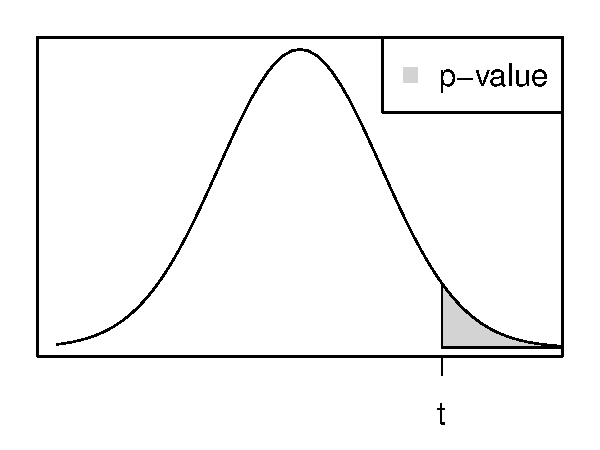
\includegraphics[scale=0.5]{figure/pvalue_upper.pdf}
\end{column}
\end{columns}
\vspace{1cm}
\end{frame}

%---------------------------------------------
\begin{frame}{Computing $p$-values}
\begin{columns}
\begin{column}{0.45\textwidth}
%\large
One-sided test (lower-tail):\\
$H_0: \mu = \mu_0$\\
$H_A: \mu < \mu_0$\\
\vspace{10pt}
Test statistic:\\
$$t = \frac{\bar{x} - \mu_0}{s/\sqrt{n}}$$\\
\vspace{10pt}

$p$-value $= \texttt{pt(t, df = n-1)}$\\ 
\vspace{10pt}
Reject $H_0$ if $p$-value $< \alpha$\\
\end{column}
\begin{column}{0.5\textwidth}
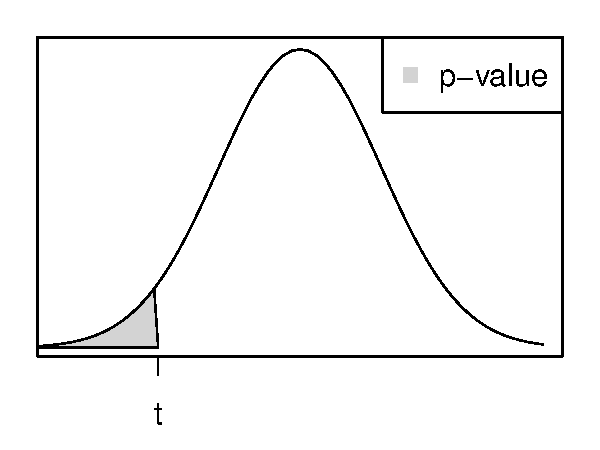
\includegraphics[scale=0.5]{figure/pvalue_lower.pdf}
\end{column}
\end{columns}
\vspace{1cm}
\end{frame}

%---------------------------------------------
\begin{frame}{Computing $p$-values}
\begin{columns}
\begin{column}{0.55\textwidth}
%\large
Two-sided test:\\
$H_0: \mu = \mu_0$\\
$H_A: \mu \neq \mu_0$\\
\vspace{10pt}
Test statistic:\\
$$t = \frac{\bar{x} - \mu_0}{s/\sqrt{n}}$$\\
\vspace{10pt}

$p$-value $= \texttt{2*pt(-abs(t), df = n-1)}$\\ 
\vspace{10pt}
Reject $H_0$ if $p$-value $< \alpha$\\
\end{column}
\begin{column}{0.45\textwidth}
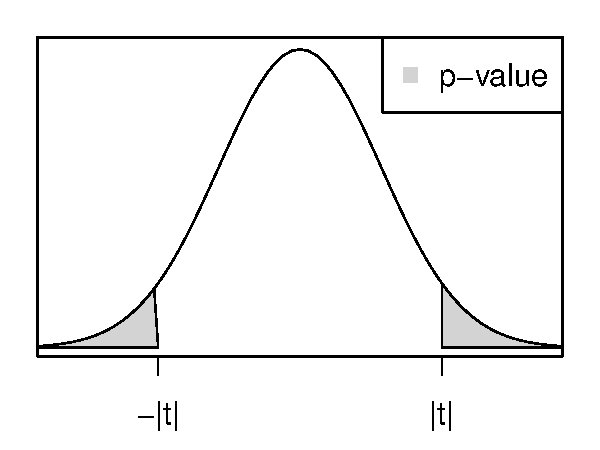
\includegraphics[scale=0.5]{figure/pvalue_both.pdf}
\end{column}
\end{columns}
\vspace{1cm}
\end{frame}

%---------------------------------------------
\begin{frame}{Conditions}
The hypothesis test is valid if the following conditions are satisfied:
\vspace{5pt}
\begin{itemize}
\item The data come from a random sample.  (This is called the \textbf{independence condition} in the textbook.)
\vspace{5pt}
\item The sample size $n$ is large ($n \geq 30$).  Otherwise, if the sample size is small ($n < 30$), the data should have an approximate normal distribution. (This is called the \textbf{normality condition} in the textbook.)
\vspace{5pt}
\item Additionally, the data should not contain any extreme outliers.
\end{itemize}
\vspace{5pt}
Graphical methods (box plots, histograms) can be used to check if the data have an approximate normal distribution when the sample size $n$ is small.\\  
\vspace{5pt}
Note that these are exactly the same conditions we check for a confidence interval.
\end{frame}

\begin{frame}{Example 1 (from \emph{Open Intro}, Chapter 7.1)}
\small
\begin{itemize}
\item Is the typical US runner getting faster or slower over time? We consider this question in the context of the Cherry Blossom Race, which is a 10-mile race in Washington, DC each spring.
\item The average time for all runners who finished the Cherry Blossom Race in 2006 was 93.29 minutes.  Using data from a random sample of 100 participants in the 2017 Cherry Blossom Race,  we want to determine  whether runners in this race are getting faster or slower, versus the other possibility that there has been no significant change.
\item Summary statistics and a histogram of the race times (in minutes) for the 2017 Cherry Blossom Race are shown below.
\end{itemize}
\begin{table}[ht]
\begin{tabular}{lll}
\hline
n & $\bar{x}$ & s\\
\hline
100 & 97.32 & 16.98
\end{tabular}
\end{table}
\begin{figure}
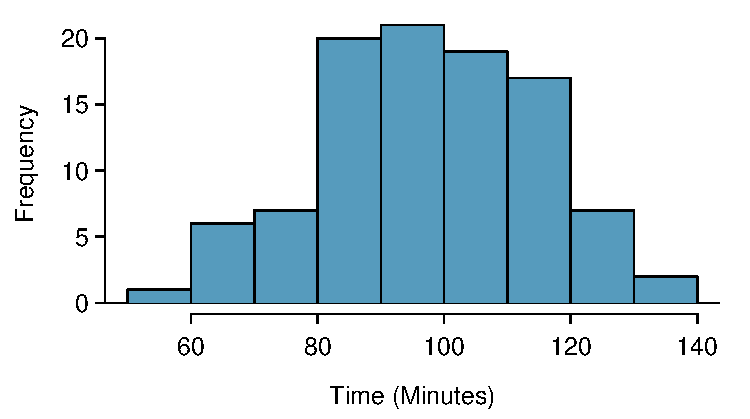
\includegraphics[scale=0.4]{figure/run17SampTimeHistogram.pdf}
\end{figure}
\vspace{5pt}

\end{frame}

\begin{frame}{Example 1}
\begin{enumerate}[(a)]
\item Write the null and alternative hypothesis for a two-sided test.
\vspace{1cm}
\item Check the conditions for the hypothesis test.
\vspace{2.5cm}
\item Calculate the test statistic.
\vspace{2.5cm}
\end{enumerate}
\end{frame}

\begin{frame}{Example 1}
\begin{enumerate}[(a)]
\setcounter{enumi}{3}
\item Calculate the $p$-value and make a decision using $\alpha = 0.05$ significance level.\\
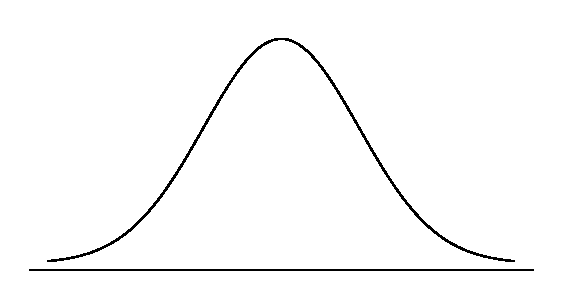
\includegraphics[scale=0.35]{figure/norm_draw.pdf}
\vspace{0.75cm}

\item What is the conclusion of the test in the context of the data?
\vspace{3.25cm}
\end{enumerate}
\end{frame}

\begin{frame}{Example 2}
Find the $p$-value for the given t-test statistic and sample size.  Also determine if the null hypothesis would be rejected at $\alpha = 0.05$.  Assume all the conditions for the hypothesis test are satisfied.
\begin{enumerate}[(a)]
\item $H_A: \mu > \mu_0$, $n=9$, $t=1.7$\\
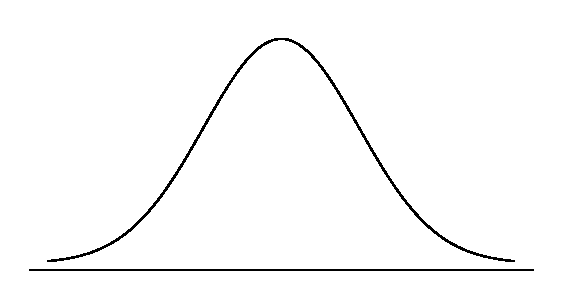
\includegraphics[scale=0.35]{figure/norm_draw.pdf}
\vspace{0.75cm}
\item $H_A: \mu \neq \mu_0$, $n=40$, $t=-3.1$\\
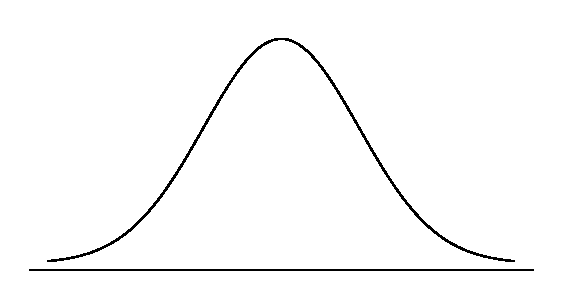
\includegraphics[scale=0.35]{figure/norm_draw.pdf}
\vspace{0.75cm}
\end{enumerate}
\end{frame}


\end{document}
